\section{Introduction: what is digitalisation?}

Wind lidar is an inherently digital measurement device in that the results of the measurement are digital signals (radial wind speed, wind vector, etc.). Similarly, wind turbines, wind plants, and the rest of the energy system infrastructure generate huge amounts of data. Digitalisation can be seen as the process whereby wind lidar data, wind energy system infrastructure data, and other data are used together to enable more reliable and more valuable energy. Together, they will enable the wind energy plant of tomorrow (Figure \ref{fig:digital_windplant}).

\begin{figure*}[!hbt]
    \centering
    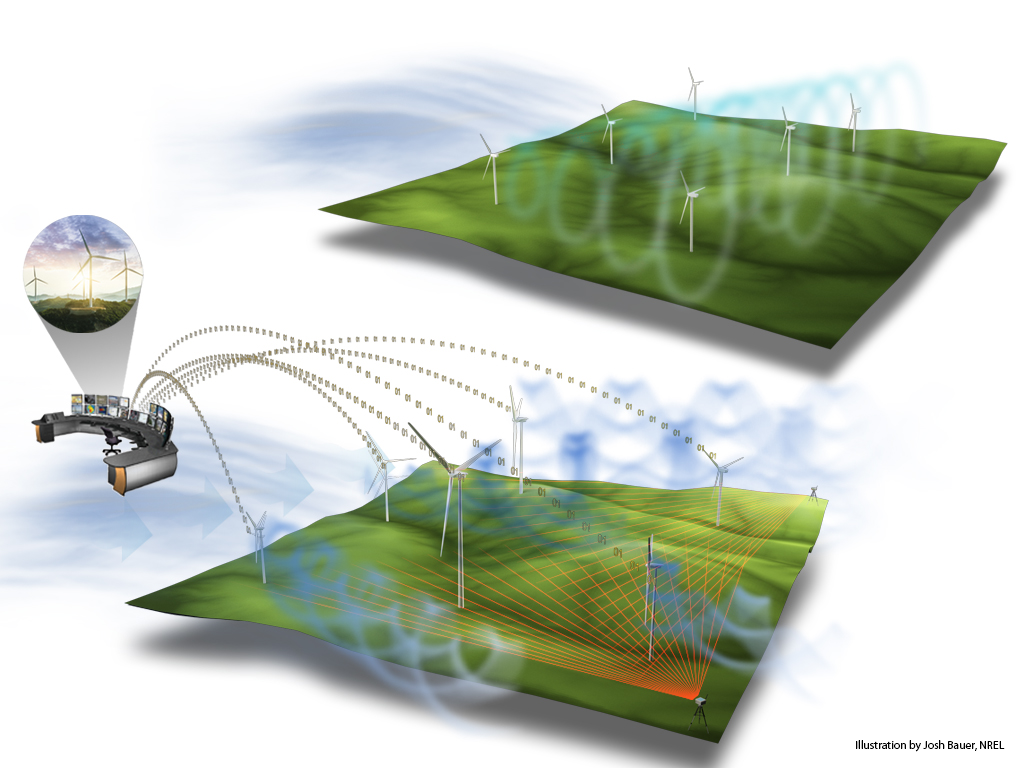
\includegraphics[width=0.85\textwidth]{figures/NRELTP-5000-68123-Fig4.png}
    \caption{Digitalisation of wind lidar and wind plants will enable the transition from the wind plant of today (top) to the networked wind plant of tomorrow (bottom). Figure courtesy Josh Bauer, NREL}
    \label{fig:digital_windplant}
\end{figure*}

However, it is difficult to know what digitalisation will involve until we have tried it. Therefore, this workshop set out to develop user stories for several different wind lidar usage scenarios. These are discussed in more detail in Section 3.